\section{Local Challenge: Passing Challenge}
\label{sec:PassingChallenge}

\subsection{Idea of the Challenge}
Teamwork is an important element in the RoboCup SPL. A fundamental teamwork component is the passing the ball between teammates. The goal of this challenge is to push teams to develop an offensive passing strategy. 

The challenge requires two active ``attacker'' robots, and two static ``obstacle'' robots (\cf Section \ref{sec:stationary_obstacle_robots}). The attackers' robots must complete as many passes between them as possible within in a 5 minute period.
A neutral referee will observe the challenge via a video stream, see \ref{sec:streaming_setup}.
Teams may make three attempts with their final score being their best attempt. Teams cannot change code between the attempts.
\begin{figure}[ht]
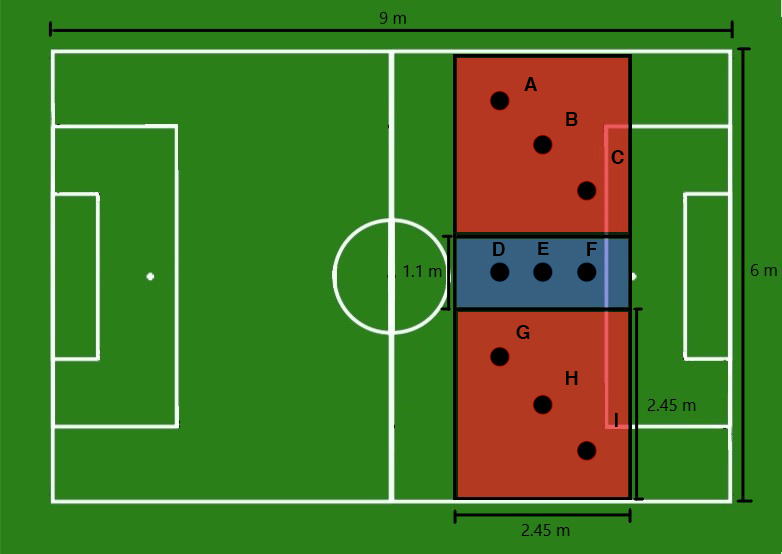
\includegraphics[width=0.95\linewidth]{figs/ch_2_full.jpg}
\caption{Setup using the standard SPL field (\cf section \ref{sec:field_dim}). The red zones are for attacking robots, and the blue zone for defending robots. }
\label{ch2:zone96}
\centering
\end{figure}

\begin{figure}[ht]
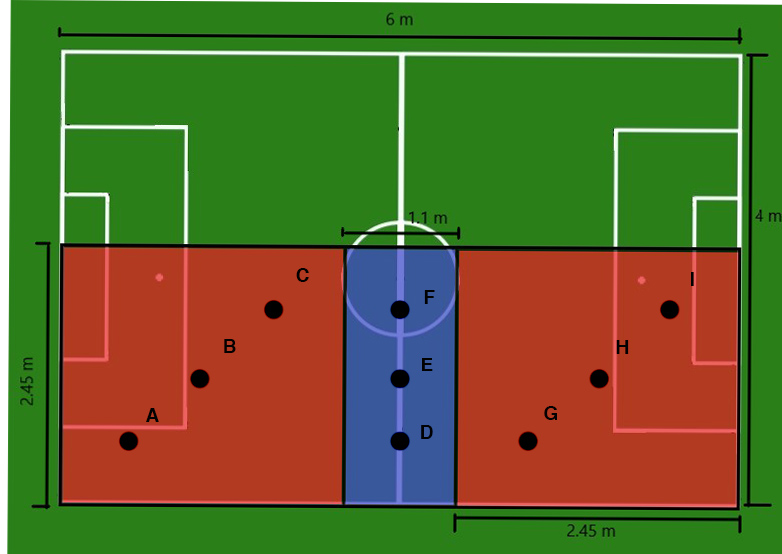
\includegraphics[width=0.95\linewidth]{figs/ch_2_reduced.jpg}
\caption{Example setup using the minimum field size (\cf section \ref{sec:field_dim}). The red zones are for attacking robots, and the blue zone for defending robots.
%The area can be applied also on fields with different dimensions, the basic requirement for the field is to be large enough to accommodate within it the areas necessary for the challenge, whose total dimensions are 6m by 2.45m.
}
\label{ch2:zone64}
\centering
\end{figure}


\subsection{Field Setup}
This challenge will be conducted within local venue of the participating team. A field of at least 3/4 size is required~(\cf Section \ref{sec:field_dim}). 
%The requirements are the presence of a half full-size field or any field capable of hosting the area required by the challenge, whose overall size is that of a rectangle measuring 6m by 2.45m.  
The challenge requires three zones shown in Figure \ref{ch2:zone96} for a standard SPL field and Figure \ref{ch2:zone64} for a minimum size field. The combined zones for the challenge \textit{must be exactly} 6m x 2.45m. This is irrespective of the actual field used and the location of the zones on the field.
The red zones represent area available to attacker robots. The blue zone represents the area where the defender robots are placed.
The three zones should be made clearly visible to observers including the referee, by demarcating them on the field through the use of a green tape. The tape must not break the regular white field lines.
Robots must localize using the regular filed lines.


\subsection{Robots positioning}
The two active robots are the attacking robots. The defending robots must be turned off and thus act like static obstacle robots (\cf Section \ref{sec:stationary_obstacle_robots})
%TODO: Common Rules reference
The starting robot's positions are identified by the points ${A,B,C,D,E,F,G,H,I}$ in Figures \ref{ch2:zone96} and \ref{ch2:zone64}.
The robot's positions are:

\textbf{Standard SPL field (Vertical setup) -} the reference frame of each point is put in the lower left corner of the corresponding area.
\\
$A = G = (0.6m, 1.8m)$
\\
$B = H = (1.2m, 1.2m)$
\\
$C = I = (1.8m, 0.6m)$
\\
$D = (0.6, 0.55m)$
\\
$E = (1.2m, 0.55m)$
\\
$F = (1.8m, 0.55m)$
\\
\\
\textbf{Reduced size field (Horizontal setup) -} the reference frame of each point is put in the lower left corner of the corresponding area.
\\
$A = G = (0.6m, 0.6m)$
\\
$B = H = (1.2m, 1.2m)$
\\
$C = I = (1.8m, 1.8m)$
\\
$D = (0.6, 0.55m)$
\\
$E = (1.2m, 0.55m)$
\\
$F = (1.8m, 0.55m)$
\\
\\
One attacking robots is randomly placed at placed in A, B, or C, and the other attacking robot randomly at G, H, or I.  One attacking robot is randomly selected to start with the ball. The defenders are positioned randomly D, E, or F.
See Figure \ref{ch2:zone96} and Figure \ref{ch2:zone64}.

\subsection{Challenge Execution}
A team may make three attempts at the challenge. For each attempt the attacking robots must be connected to GameController.
Before each attempt, GameController is set to Initial. After the robots are positioned, the GameController changes to Ready state and then Set. The attempt commences using the referee whistle and GameController process, as in typical SPL games~(\cf Section~\ref{sec:game_process}). 

The attacking robots pass the ball back-and-forth as often as possible until the attempt ends. The attackers can leave their respective red starting zones for up to 30 seconds, which may be necessary in cases where the ball is near (or at) the edge of the red zone.

If the ball leaves the red zone (such as from a bad pass), then the ball is manually put back at the edge of the red zone where it went out. This is similar to placing the ball for a kick-in in a soccer game~(\cf Section~\ref{sec:kick_in}).  If the ball went out from a blue zone, it is put back at position A or G, corresponding to the last red zone in which the ball was located.
    
An attempt ends when: 
\begin{enumerate}
    \item The timeout is reached,
    \item The defenders touch the ball,
    \item One attacking player stays out of its red starting zone for more than 30 seconds.
\end{enumerate}

Each team may make three attempts at the challenge however, they cannot modify their code between the attempts.

\subsubsection{Passing definition}
\label{sec:pass-definition}
A successful pass is defined as:
\begin{enumerate}
    \item The ball has been touched by two attacking robots.
    \item The ball moved more than one meter from its starting position.
    \item The ball crosses the blue zone so that is starts and ends in different red zones.
    \item The ball stops moving in a red zone.
\end{enumerate}

\subsection{Scoring and Overall Ranking}
One point is awarded for each successful pass (\cf Section~\ref{sec:pass-definition}). The neutral referee will count and adjudicate successful passes. The score for an attempt is the total number of successful passes.

A team is given a final score that is the best of their three attempts. Teams are ranked overall by their score, from the highest to the lowest. 
